\chapter{Introduction to \cognicryptsast{} and \codyze}
\label{ch:intro}
In this chapter, we will discuss \cognicryptsast{} and \codyze{} in greater detail to gain a better understanding of the tools and their capabilities. In addition, this information can be utilized to compare the tools in Chapter \ref{ch:compare} and to evaluate their performance in Chapter \ref{ch:eval}.

\section{\cognicryptsast}
\cognicryptsast{} \cite{stefanphd} is an open-source static analyzer that analyses Java codes to find misuses of cryptographic APIs. \cognicryptsast{} is integrated into the \cognicrypt{} Eclipse plugin and can also be used as a standalone command-line tool to analyze Android and Java applications \cite{cryptoanalysis}. \cognicryptsast{} consumes \crysl{} \cite{skm19} rules to configure a flow-sensitive and context-sensitive static data-flow analysis. Flow-sensitivity is the ability to determine the order in which statements are presented \cite{pointer}. The context-sensitive analysis is an inter-procedural analysis that considers the calling context when analyzing a method \cite{pointer}. An intra-procedural analysis analyzes a single procedure, while an inter-procedural analysis examines the interrelationships among procedures. Data flow analysis refers to the process of tracking data through a program in order to explain its behavior without actually executing the program \cite{johannesphd}. According to Krueger \cite{stefanphd}, \cognicryptsast{} is also field-sensitive but not path-sensitive. Path-sensitive data flow analysis improves the precision of data flow analysis by analyzing the feasibility of paths \cite{pathsensitive}.

\cognicryptsast{} uses the Soot framework \cite{soot} for static analysis. Soot enables Java developers to build their own static analyzer tool. It contains several intra-procedural and inter-procedural features to solve intra- and inter-procedural analysis problems. Direct analysis of Java bytecode can be hindered by the unclarity of data flow; hence \cognicryptsast{} employs Soot that offers several intermediate representations (IR) of Java code. Jimple is the fundamental Soot IR that simplifies analyzing and making a graph. \cognicryptsast{} builds a Call Graph (CG) from Jimple code. A call graph is a directed graph that represents the calling relation in a program function. Nodes represent methods, and edges represent a call relation between two methods \cite{callgraph}. In addition, analysis employs CFGs to identify the control flow of each method. For performing inter-procedural analysis of a complete program, the \cognicryptsast's analysis combines individual control flow graphs and the program's call graph in order to construct an inter-procedural control flow graph (ICFG).

\cognicryptsast{} utilizes CryptoAnalysis to build CGs and perform the analysis. CryptoAnalysis is a compiler that translates rules to static analysis. CryptoAnalysis warns the developer if any part of the specified \crysl{} rules is violated in the code. Three different static sub-analyses form CryptoAnalysis: typestate analysis, a Boomerang \cite{boomerang} instant and taint analysis for Android applications. Typestate analysis checks the valid sequence of operations based on the defined order on \crysl{} rules. For instance, the call sequence of the KeyGenerator object is \code{getInstance}, \code{init} (optional), and then \code{generatekey} (see Listing \ref{lst:orgkeygencrysl} Line \ref{line:ordercrysl}). Any other combinations will be false. CryptoAnalysis uses Boomerang, a demand-driven pointer analysis for Java, to extract parameters on the fly to check them against the defined \crysl{} rules. For example, it checks if a valid \code{algorithm} is chosen for the \code{getInstance} method of KeyGenerator.
Cryptoanalysis also includes taint analysis, which detects flaw injections or leaks of sensitive information. For analyzing Android applications, CryptoAnalysis employs Flowdroid \cite{flowdroid} which is a static taint analysis for Android applications.

It is possible to select different kinds of CG algorithms from \cognicryptsast, CHA (Class Hierarchy Analysis), SPARK \cite{spark} and SPARK\_LIBRARY that are available through command-line commands or Eclipse preference pages. The CHA is the default algorithm, which is not precise but is efficient. SPARK is a framework for call graph construction and points-to analysis, and it is a part of the Soot framework. SPARK's call graph construction algorithm considers any call that may occur at any point in the execution of the program \cite{soot}. SPARK implements a context-insensitive points-to analysis. The points-to analysis associates variables with the allocation sites \cite{pointer}. An analysis that is context-insensitive merges all call sites of a procedure.
SPARK\_LIBRARY is a SPARK mode specifically designed for the analysis of libraries. For all classes within the library, dummy allocation sites are instantiated, resulting in non-empty points-to sets for variables within the library \cite{johannesphd}. 

Misuses in \cognicryptsast{} are categorised into 7 categories, namely, ConstraintError, NeverTypeOfError, ForbiddenMethodError, ImpreciseValueExtractionError, TypestateError, RequiredPredicateError, IncompleteOperationError \cite{cryptoanalysis}. The error messages that \cognicryptsast{} generates depend on the type of misuse and will be automatically generated at the end of the analysis.
\label{sec:cc}

\section{\codyze}
As of the date of this thesis, there have been no papers published on \codyze{}, and the documentation page is brief \cite{cod}. Therefore, to understand \codyze{}, we investigated its source code on Github \cite{codyzegit}, its documentation page and consulted with one of \codyze's developers (personal communications with one of the \codyze's developers via several emails and an online meeting on Sep 17, 2021).

\codyze{} \cite{cod} is an open-source static analysis tool for Java, C and C++ programs developed by Fraunhofer AISEC\footnote{https://www.aisec.fraunhofer.de/}. It generates a code property graph (CPG) \cite{cpg} from the source code and analyzes it against predefined \MARK{} \cite{cod} rules for finding cryptographic misuses. \MARK{} is a domain-specific language (DSL) designed to write correct usages of Java, C, and C++ cryptographic APIs. Code property graphs allow \codyze{} to handle non-compiling or incomplete code. A CPG is a directed multigraph, which means that two nodes may be connected by multiple edges. Listing \ref{lst:sampleCCPG} illustrates an example code that shows a source method leaking (potentially) sensitive data and a sink method that may expose the data. Figure \ref{fig:CPG} depicts a CPG representation of Listing \ref{lst:sampleCCPG}, in which there are multiple edges between the nodes PRED and DECL. The nodes represent program constructs. For example, in figure \ref{fig:CPG}, PRED is a predicate node that indicates the condition of the if statement in Listing \ref{lst:sampleCCPG}, Line \ref{line:PRED} and DECL refers to the declaration statements of Line \ref{line:DECL} in the Listing \ref{lst:sampleCCPG}.
This graph incorporates the properties of Abstract Syntax Tree (AST), Control Flow Graph (CFG), and Program Dependence Graph (PDG) in a single data structure \cite{cpg}. An AST represents the abstract syntactic structure of the source code. It is an ordered tree with inner nodes representing operators and leaf nodes representing operands \cite{cpg}. A CFG is a graph that represents all the possible paths that can be traversed during program execution. It is a directed graph that explicitly describes the order in which code statements are executed as well as conditions that need to be met for a particular path of execution to be taken \cite{controlflowgraph}. The program dependence graph indicates explicit dependencies between statements and predicates. Vertices in PDG represent the statements and predicates in the program. The edges representing the dependencies between components fall into two categories; data dependency edges reflect the influence of one variable upon another, and control dependency edges reflect the influence of predicates on the values of variables. After constructing each graph individually, the three graphs are merged to form the CPG. Graph nodes are the same as AST nodes, edges and labels are combinations of all three graphs, and sets of property keys and property values for nodes and edges are from AST and PDG graphs. Property keys and values as well as labels on AST edges are not shown in Figure \ref{fig:CPG}. CFG and PDG edges are indicated by colors.


\begin{lstlisting}[caption= Code example for making it into a CPG \cite{cpg}. , label={lst:sampleCCPG}, backgroundcolor =  , xleftmargin=.3\textwidth, frame = single, xrightmargin=.3\textwidth, escapechar=|]
void foo() 
 {  
    int x = source(); 
    if (x < MAX) |\label{line:PRED}|
    { 
        int y = 2 * x; |\label{line:DECL}|
        sink(y); 
    } 
}

\end{lstlisting}
\begin{figure}[H]
\centering
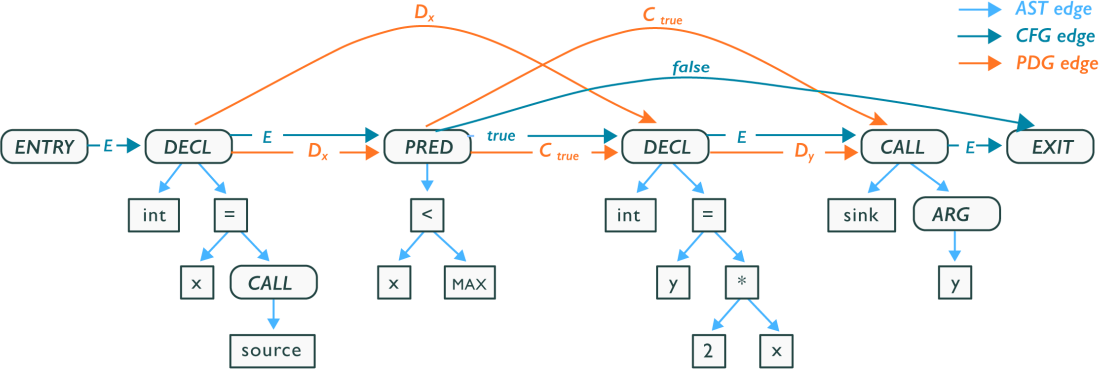
\includegraphics[width=1\linewidth]{figures/cpg-original.png}
\caption{Code property graph for code sample in Listing \ref{lst:sampleCCPG} \cite{cpg}.}
\label{fig:CPG}
\end{figure}

Observing \codyze's source code, we discovered that \codyze{} is a flow-sensitive static data-flow analysis. Through the use of CPGs and graph traversals, \codyze{} is able to access the code flow and data dependencies associated with each node, thereby providing a data-flow analysis and can check the nodes in the CPG (e.g., methods, variables, etc.) against the defined \MARK{} rules. In addition, there are \MARK{} rules that specify the correct order of using an API's methods\footnote{\url{https://github.com/Fraunhofer-AISEC/codyze/blob/0468af19b90b16353402938db4e326b6dc63c4f7/src/dist/mark/bouncycastle/RulesBase_Cipher.mark}}, which indicates that \codyze{} is flow-sensitive. CPG and the query language are not enough to determine whether the program complies with the \MARK{} order rules, so \codyze{} developers implemented an intra-procedural typestate analysis. By using typestate analysis, \codyze{} determines whether a sequence of operations is valid based on the \MARK{} rules\footnote{\url{https://github.com/Fraunhofer-AISEC/codyze/blob/e67d5fa0a1c956ce4be53fcdecf1990eb8dfb430/src/main/java/de/fraunhofer/aisec/codyze/analysis/wpds/TypestateWeight.java}}.
CPG does not cover inter-procedural analysis \cite{cpg}. Further, it is stated in the Java documentation for \codyze's implementation of typestate analysis that it is not inter-procedural; Thus, \codyze{} is not considered to be inter-procedural. Nevertheless, when evaluating \codyze's performance, we discovered that \codyze{} is partially inter-procedural. At the time of this thesis, no published papers about \codyze{} were available; therefore, we were unable to identify any other properties of it. However, we can better assess the analysis properties of \codyze{} through evaluation of its analysis of example codes. We will discuss it further in the evaluation chapter (cf. Chapter \ref{ch:eval}).


\codyze{} runs in three modes, interactive command line, non-interactive command line, and as a server for Language Server Protocol (LSP) \cite{lsp}. \codyze{} uses the LSP in order to provide greater flexibility in the use of different IDEs and supporting several languages. The LSP describes the communication protocol used between an editor or IDE and a language server, which enables features such as auto-complete, go to definition, etc. With a standard communication protocol, a single language server can be re-used in various code editors without too much effort \cite{lsp}. \codyze{} creates a language server that converts the source code from a client (IDE or command line) to a CPG. \codyze{} developers have implemented a parser that parses \MARK{} rules into a model that the analysis server can use. The analysis server analyzes the CPG against the \MARK{} model with the help of Crymlin queries \cite{gremlin}. Crymlin is an extension of the Apache Gremlin graph traversal language that provides a variety of shortcuts for searching through code property graphs \cite{gremlin}. 


\codyze{} also provides a JSON file (findingDescription.json) that contains all the possible errors based on the \MARK{} rules in a human-readable format and is stored in the same location as the \MARK{} rules (Listing \ref{lst:findings}). This file may later be used to create error messages in the client. It contains all possible errors, with the exception of errors related to the incorrect order of method calls and the use of insecure methods. The error messages for these two violations are generated automatically at runtime, since the error message for the first violation (the incorrect order) contains the missing methods\footnote{\url{https://github.com/Fraunhofer-AISEC/codyze/blob/0468af19b90b16353402938db4e326b6dc63c4f7/src/main/java/de/fraunhofer/aisec/codyze/analysis/markevaluation/OrderNFAEvaluator.java}} and the message for the second violation contains the forbidden call\footnote{\url{https://github.com/Fraunhofer-AISEC/codyze/blob/04b5db6029a1bc6f8ad680cfecc796f408705031/src/main/java/de/fraunhofer/aisec/codyze/analysis/markevaluation/ForbiddenEvaluator.kt}}.

Listing \ref{lst:findings} shows a sample error description in the findingDescription JSON file generated by \codyze{}. The error refers to the incorrect cryptographic algorithm or the absence of an algorithm during the creation of the Cipher object. The first line (Line \ref{line:errorname}) is the name of the error. HelpUri (Line \ref{line:helpuri}) contains a URL from which \MARK{} rules are derived (Bundesamt für Sicherheit in der Informationstechnik\footnote{Federal Office for Information Security} or BSI \cite{BSI}). FullDescription (Line \ref{line:fulldesc}) provides a complete description of the error, while shortDescription (Line \ref{line:shortdesc}) is only a concise description. Line \ref{line:fixes} describes the possible solutions to the problem. The fix, in this case, is to use the AES or RSA algorithm.
\pagebreak
\begin{lstlisting}[language=json, caption= {Part of findingDescription.json file generated by \codyze{} after analyzing Listing \ref{lst:codesample}}, label={lst:findings}, escapechar=@]
...
{
    ...
    "Invalid_TR21021_Cipher": { @\label{line:errorname}@
    "helpUri": "https://www.bsi.bund.de/SharedDocs/Downloads/DE/BSI/Publikationen@\label{line:helpuri}@
    /TechnischeRichtlinien/TR02102/BSI-TR-02102.pdf",
    "fullDescription": {@\label{line:fulldesc}@
      "text": "A cipher was detected that does not match one of the recommended ciphers by BSI TR-02102. Use of weak or unspecified ciphers may not guarantee sufficient security."
    },
    "shortDescription": {@\label{line:shortdesc}@
      "text": "Use of an unspecified cipher"
    },
    "fixes": [@\label{line:fixes}@
      {
        "description": {
          "text": "Use AES as symmetric-key (cf. 2.1) or RSA for asymmetric-key algorithm (cf. 3)"
        }}]
    }
    ...
 }
 ...
\end{lstlisting}


As well as spotting cryptographic misuses in a program, \codyze{} will also alert if a \MARK{} rule is being used correctly. \codyze{} can be used as a console application or integrated into IDEs or CI pipelines. In the time of this thesis, \codyze{} is integrated into Eclipse, Visual Studio, and IntelliJ \cite{cod}. \codyze{} offers a standard Python console for exploring the source code project using the Crymlin query interface.


\label{sec:codyze}

\setlength{\parindent}{0em}
\setlength{\parskip}{2em}
\par
Here we have described how \cognicryptsast{} and \codyze{} perform the analysis, the components they use to accomplish it, and the properties of their analysis. Having an understanding of \codyze{} and \cognicryptsast, we can now begin to compare them. In the following chapter, we will provide a comparison of these tools.

